% !TeX spellcheck = en_US
\chapter{Solution Approach}  \label{chap:four}%%

The 2D object detector of Providentia Mono3D currently relies on YOLOv7 pre-trained on COCO dataset. It downscales the incoming frames from 1920x1200 to 1280x1280 or even 640x640 (with padding) to speed up the process to meet the system's real-time requirement. However, this downscaling sacrifices detection accuracy, particularly for small objects farther away from the camera. Moreover, the COCO dataset annotates eighty classes, but only six classes overlap with our TUM Traffic dataset. The Providentia 2D detector filters six COCO sub-classes: CAR, BUS, TRUCK, MOTORCYCLE, BICYCLE, and PEDESTRIAN. The VAN, TRAILER, EMERGENCY\_VEHICLE, and OTHER classes from the A9 Dataset cannot yet be recognized. This poses some limitations. Firstly, occlusion with classes that are not considered in our dataset will cause big blobs in the detected mask. Secondly, the classes TRAILER, VAN, EMERGENCY\_VEHICLE, and OTHER are not included in COCO and will either not be detected or detected with another class label. 

To address these limitations, in this work, we fine-tune the models on our TUM Traffic Intersection dataset. This approach not only addresses class mismatches but also improves detection by training models to understand our camera's perspective, considering factors such as view angle and distance. However, since the TUM Traffic dataset lacks segmentation labels, additional steps are required to extend the dataset with segmentation annotations.

This chapter elaborates on all the steps taken to achieve the aforementioned goals. Firstly, different state-of-the-art segmentation models are adapted to perform inference on the TUM Traffic Intersection dataset using publicly available pre-trained model weights on COCO and KINS datasets in \Cref{sec:sota_review}. This provides insights into the general performance and limitations of the models and pre-trained datasets. Subsequently, \Cref{sec:extend_annotation} outlines the process of extending the TUM Traffic dataset labels with 2D visible and amodal instance segmentation masks and bounding boxes. This section is divided into subsections, beginning with an introduction to the structure of the newly extended OpenLABEL label format (\Cref{sec:extended_openlabel_format}). Following this, a description of a simple 2D annotation interpolation pipeline is presented in \Cref{sec:2d_interpolation_pipeline} to speed up the annotation process. The annotation procedure for frames is then described in detail in \Cref{sec:mask_annotation}. Finally, \Cref{sec:object_detection_with_yolov8} delves into the training of five different YOLO and C2F models and discusses their effectiveness.

\section{Pre-trained Models on TUMTraf Intersection Dataset} \label{sec:sota_review}

\begin{figure}[htb]  
	\centering
	\begin{subfigure}{0.40\textwidth}
		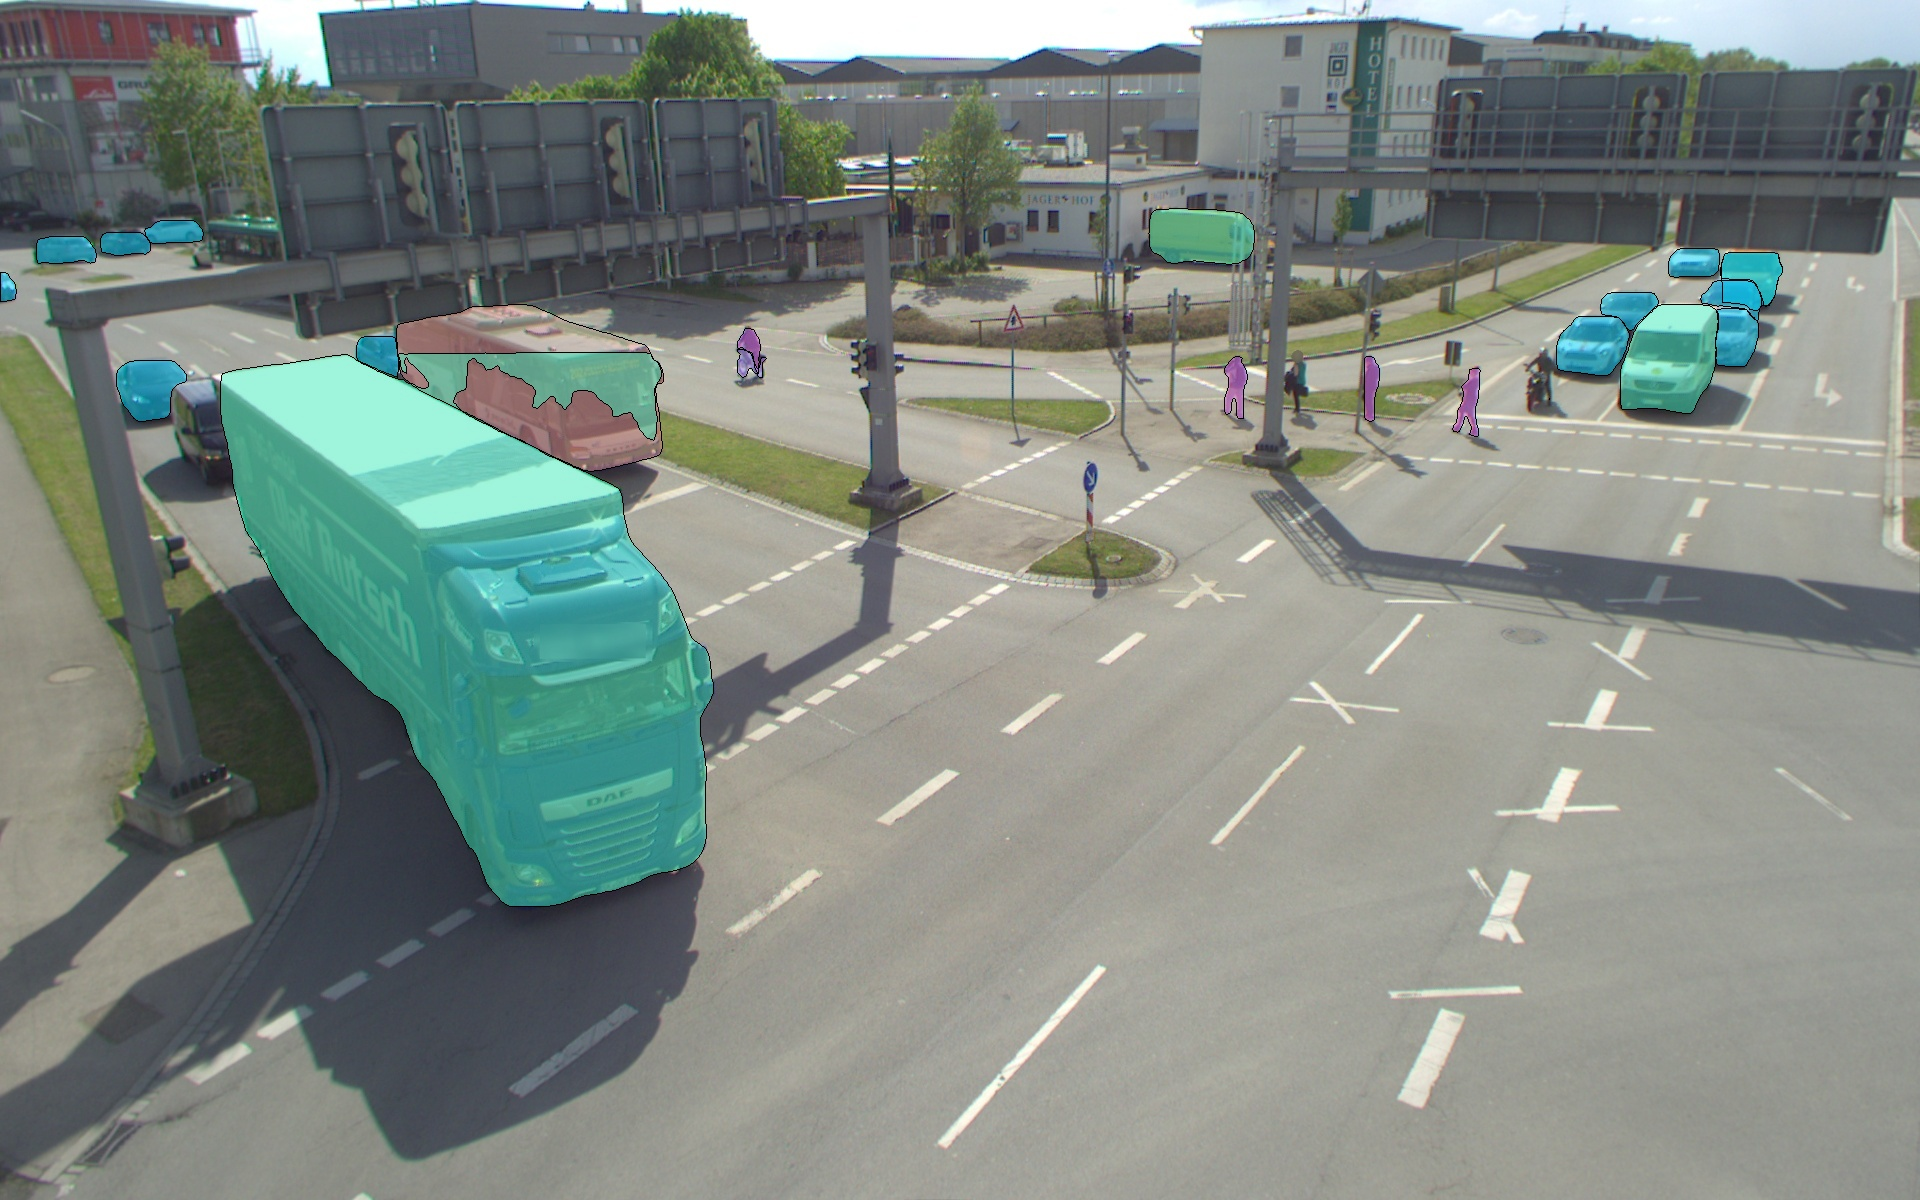
\includegraphics[width=\linewidth]{intro_yolov7.jpg}
		\caption{YOLOv7}
	\end{subfigure}
	\begin{subfigure}{0.40\textwidth}
		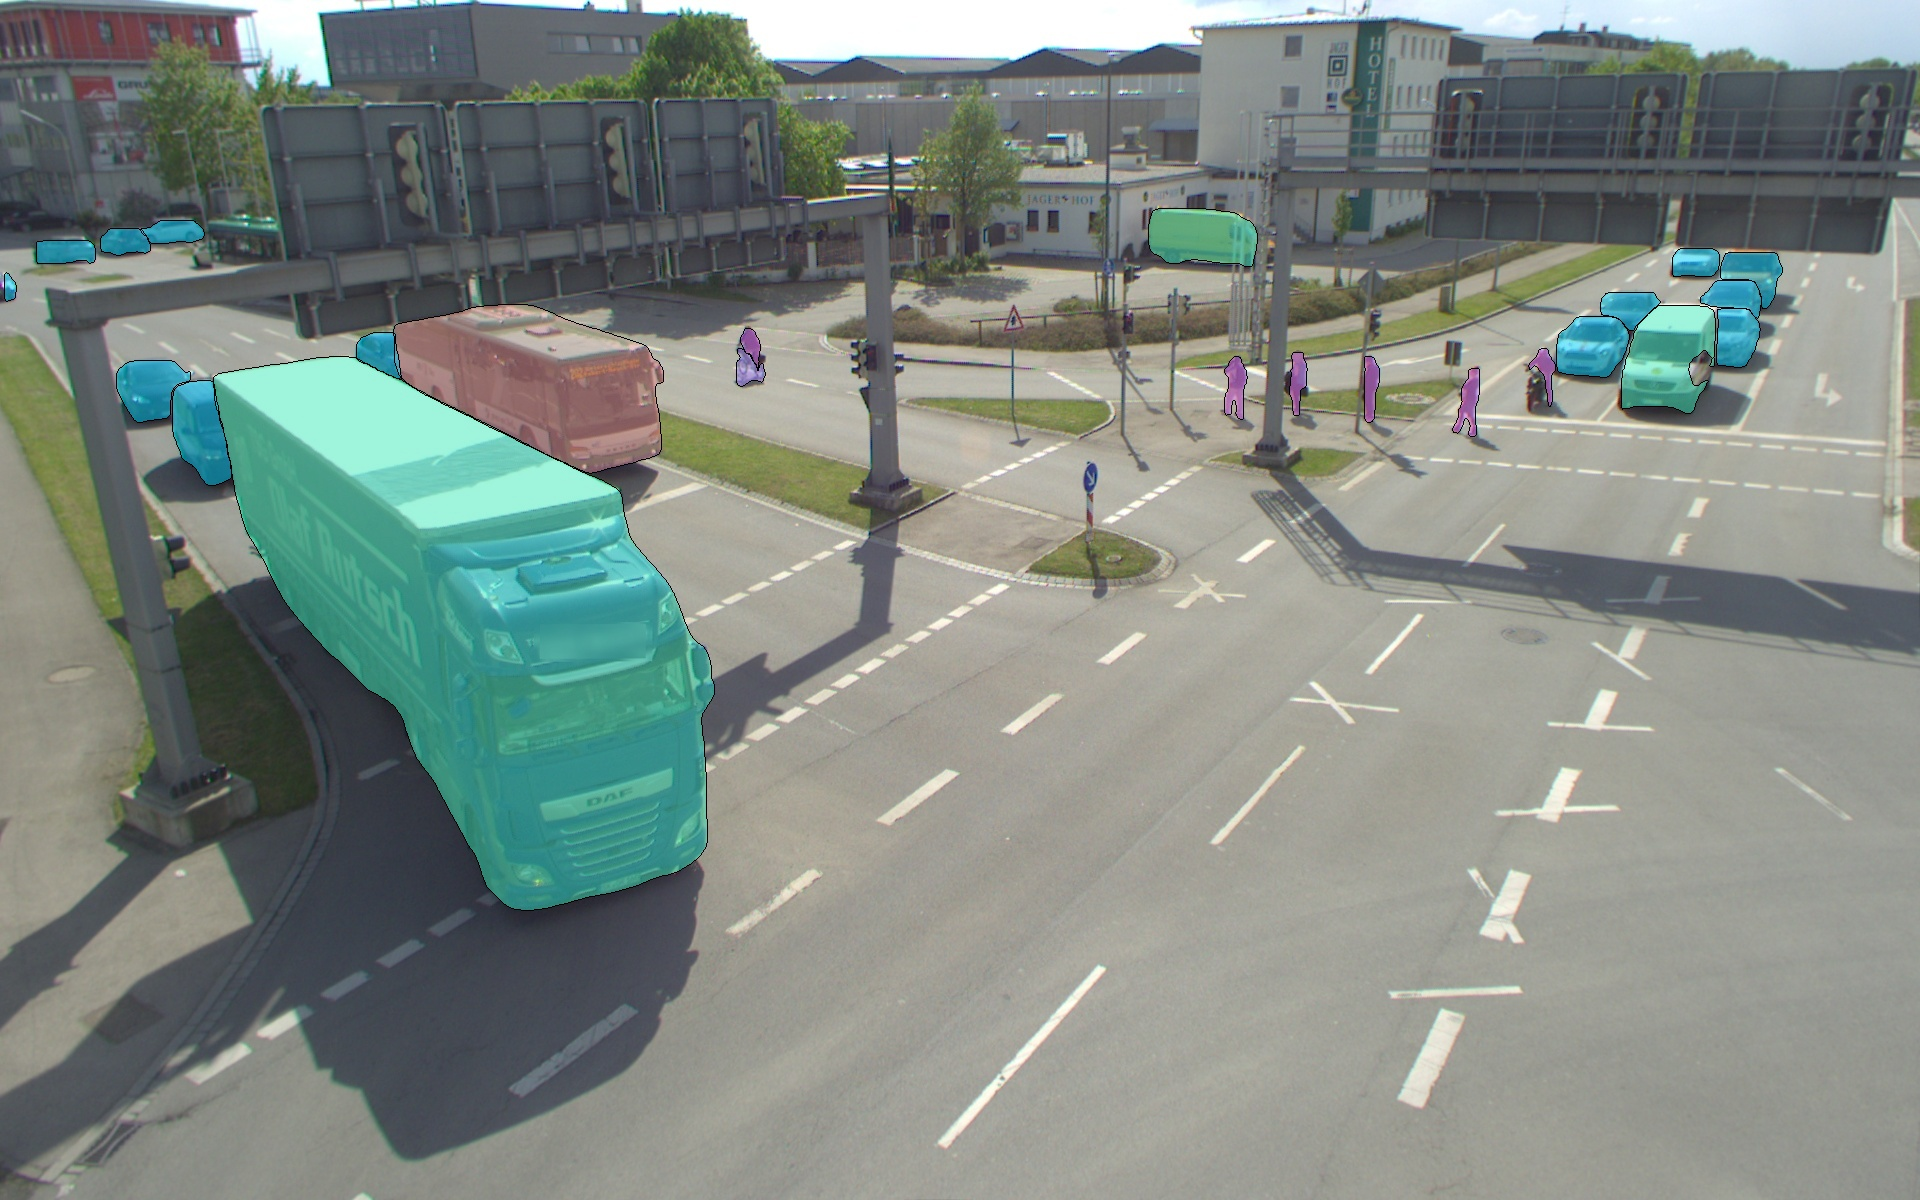
\includegraphics[width=\linewidth]{intro_yolov8.jpg}
		\caption{YOLOv8}
	\end{subfigure}
	\begin{subfigure}{0.40\textwidth}
		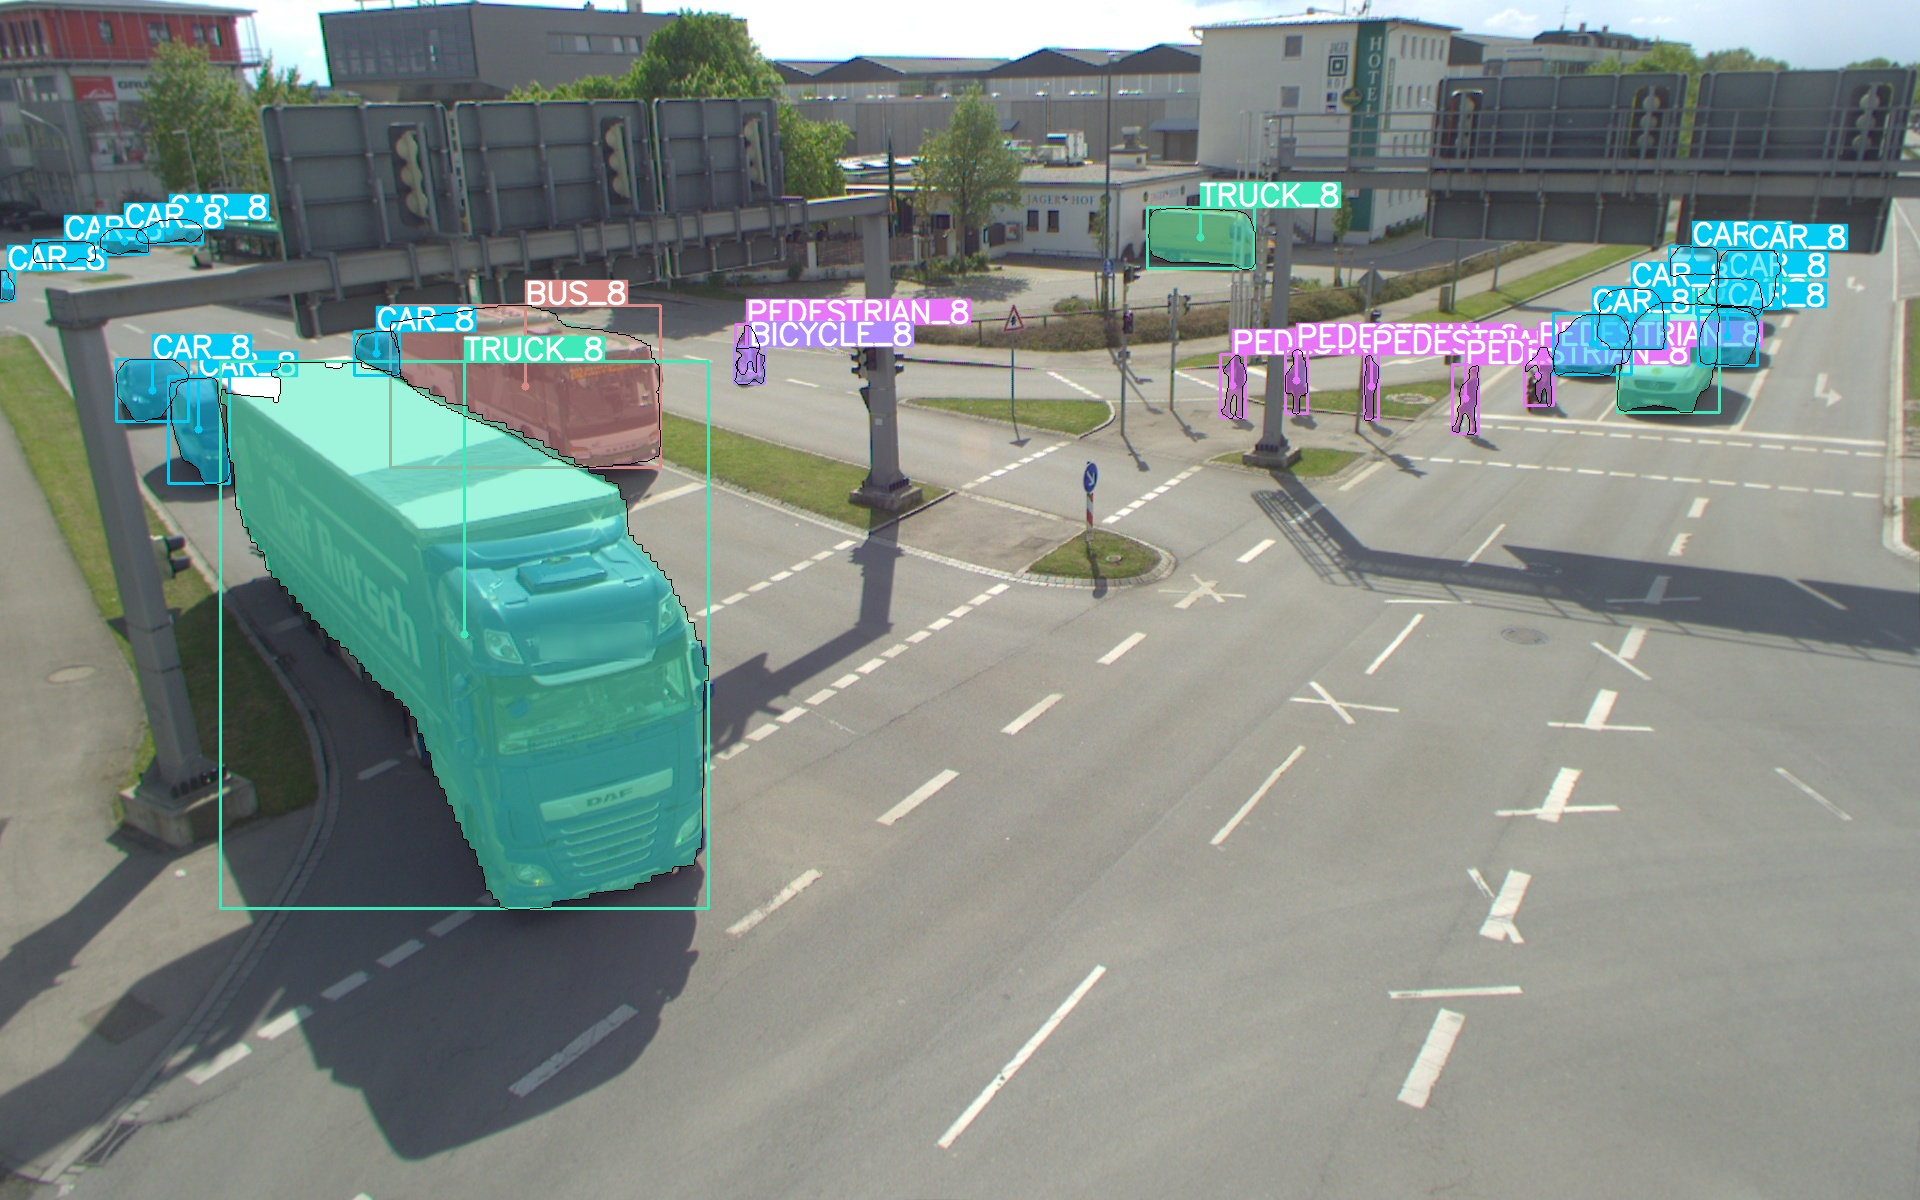
\includegraphics[width=\linewidth]{intro_c2f.jpg}
		\caption{C2F}
	\end{subfigure}
	\begin{subfigure}{0.40\textwidth}
		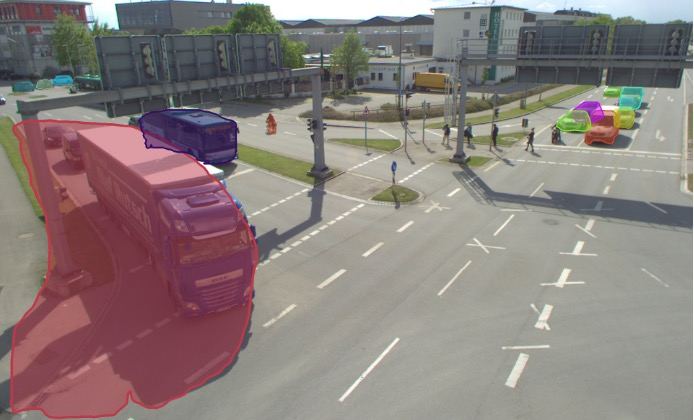
\includegraphics[width=\linewidth]{intro_walt.jpg}
		\caption{WALT}
	\end{subfigure}
	\begin{subfigure}{0.40\textwidth}
		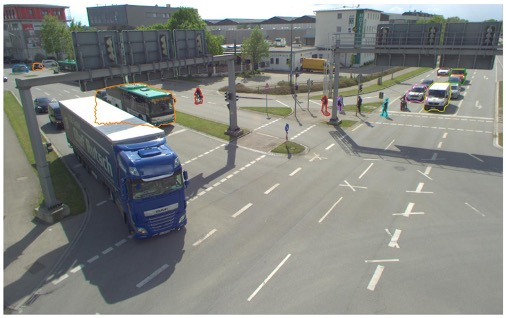
\includegraphics[width=\linewidth]{intro_e2ec.jpg}
		\caption{E2EC}
	\end{subfigure}
	\begin{subfigure}{0.40\textwidth}
		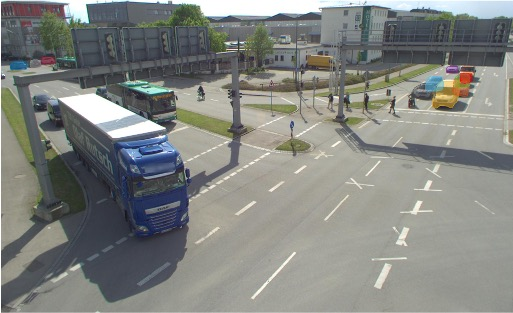
\includegraphics[width=\linewidth]{intro_aisformer.jpg}
		\caption{AISFormer}
	\end{subfigure}
	\caption{Illustration of YOLOv7, YOLOv8, C2F\_Seg, WALT, E2EC, and AISFormer models on an image in the TUMTraf Intersection dataset. YOLOv7 and YOLOv8 were trained on the COCO dataset; C2F, WALT, E2EC, and AISFormer were trained on the KINS dataset.}
	\label{figure:compare_sota_is_ais}
\end{figure}

After reviewing the literature for state-of-the-art modal and amodal instance segmentation models, promising and suitable models with publicly available pre-trained weights are chosen and adapted to perform inference on the TUMTraf Intersection Dataset. The models have been either pre-trained on COCO/COCOA or KITTI/KINS datasets. \Cref{figure:compare_sota_is_ais} and \Cref{tab:compare_sota_is_ais} demonstrate the results obtained from the instance segmentation models YOLOv7 and YOLOv8, alongside the amodal instance segmentation models C2F\_Seg, WALT, E2EC and AISFormer, on an image taken from TUM Traffic Intersection Dataset. The two YOLOv7 and YOLOv8 shown here were trained on COCO dataset, while the weights of the other four AIS models were trained on the KINS dataset. For a fair comparison, C2F\_Seg receives as input the visible detections of YOLOv8 and is, therefore, just an amodal detection extension of the IS model YOLOv8.

\begin{table}[htb]%
	\centering%
	\begin{tabular}{p{3cm} p{2cm} p{9cm}}
		\toprule
		\textbf{Model} & \textbf{\# person} & \textbf{\# vehicle} \\
		\midrule
		\code{Ground Truth} & 6 & 19 \small{(16 cars/vans, 1 motorcycle, 2 buses, 1 truck, 1 bicycle)} \\
		\code{YOLOv7\_coco} & 4 & 16 \small{(10 cars, 1 motorcycle, 1 bus, 4 trucks)} \\
		\code{YOLOv8x\_coco} & 6 & 19 \small{(13 cars, 1 motorcycle, 1 bus, 3 trucks, 1 bicycle)} \\
		\code{C2F\_Seg}&  6 & 19  \\
		\code{WALT} & 1 & 11 \\
		\code{E2EC}  & 4 & 8 \\
		\bottomrule
	\end{tabular}
	\caption{Number of detections generated from the inference of YOLOv7, YOLOv8, C2F\_Seg, WALT, E2EC, and AISFormer models, as shown in \Cref{figure:compare_sota_is_ais}. The 'Ground Truth' denotes the actual count of persons and vehicles present. The YOLO models, particularly YOLOv8 trained on COCO, exhibit the highest detection rates. E2EC and AISFormer encounter challenges in detecting large objects, while WALT faces difficulties in identifying pedestrians.}
	\label{tab:compare_sota_is_ais}%
\end{table}

Overall, the results on the TUMTraf Intersection Dataset show that IS models pre-trained on COCO can detect more objects than AIS models pre-trained on KINS. The advantage of COCO, with its larger dataset containing 2.5 million labeled objects, has likely contributed to the higher detection rate. Additionally, YOLOv8 outperforms its predecessor, YOLOv7. E2EC and AISFormer struggle to detect large objects, possibly due to being trained on frames with smaller resolutions. 

Furthermore, the YOLO models are one-stage object detection models and are much faster in inference, especially after being exported to TensorRT. In contrast, the AIS models require longer inference times and are thus not suitable for real-time detection. Detailed analysis results of inference speeds are provided in \Cref{sec:inference_speed}.

\section{Segmentation Annotation for TUMTraf Intersection Dataset}  \label{sec:extend_annotation}

The TUM Traffic dataset provides 3D bounding box labels but lacks segmentation masks. Therefore, it cannot be directly used to train instance segmentation models. To address this limitation, this work extends the TUM Traffic Intersection dataset by annotating visible and full instance masks and bounding boxes. Additionally, we adjust the OpenLABEL annotation schema of the TUMTraf dataset to accommodate these new annotations. 

\subsection{Extended Annotation Formats}  \label{sec:extended_openlabel_format}

\subsubsection{Extended OpenLABEL Format}  

First of all, we extend the OpenLABEL annotation format, described in \Cref{section:openlabel}, of the TUM Traffic dataset to include additional full instance segmentation annotations. Each "object\_data" now includes additional "bbox" and "poly2d" attributes containing two bounding boxes and polygons. The visible and amodal bounding boxes and masks are differentiated by the "full\_..." and "visible\_..." name attributes. We describe the instance masks by the bounding coordinates around the mask areas. The structure of one extended annotated object is shown in Listing 4.1. 

\begin{lstlisting}[language=json, caption={Illutration of the extended OpenLABEL Annotation JSON Structure}]
	"<object_id>" : {
		"object_data": {
			"name" : <str>, 
			"type" : <str>, 
			"cuboid" : {<...>},
			"bbox" : [ 
			{
				"name": "full_bbox",
				"val": <[x_center, y_center, width, height]>
			}, 
			{	
				"name": "visible_bbox",
				"val": <[x_center, y_center, width, height]>
			}
			], 
			"poly2d" :[ 
			{
				"name": "full_mask",
				"val": <[x1, y1, x2, y2, x3, y3, ...]>
			}, 
			{	
				"name": "visible_mask",
				"val": <[x1, y1, x2, y2, x3, y3, ...]>
			}
			] 
		}
	}
\end{lstlisting}

\subsubsection{Extended COCO Format}  

For compatibility with the CVAT labeling tool, which does not support the OpenLABEL format, we convert labels to and from COCO format for importation into and exportation out of CVAT. Inspired by the annotation structure of the KINS dataset, we also extend the COCO annotation format to store the additional amodal segmentation labels. The structure of one extended object annotation is shown in Listing 4.2. The modifications involve replacing the single "segmenation" attribute with two separate "i\_segm" and "a\_segm" attributes describing the visible (inmodal) and full (amodal) instance masks. The attributes "area" and "bbox" are replaced by "a\_area", "i\_area", "a\_bbox" and "i\_bbox" accordingly. Here, we also describe the instance masks by the bounding coordinates around the mask areas to ease the conversion to and from our OpenLABEL format. Additionally, the "iscrowd" attribute is set to 0, indicating that the annotation refers to a single object.

\begin{lstlisting}[language=json, caption={Illutration of the extended COCO Annotation JSON Structure}, keepspaces=true] 
	annotation  {
		"id"         : <int>, 
		"image_id"   : <int>, 
		"category_id": <int>, 
		"i_segm"     : <[polygon]>, 
		"a_segm"     : <[polygon]>, 
		"i_area"     : <float>, 
		"a_area"     : <float>, 
		"i_bbox"     : <[x_min,y_min,width,height]>, 
		"a_bbox"     : <[x_min,y_top_min,width,height]>, 
		"iscrowd"    : <0> 
	}
\end{lstlisting}

\subsection{Annotation Format Converters}  \label{sec:format_converters}

Different stages of the work requires different label formats. In particular, YOLOv8 mandates data labels in YOLO format with a specific folder structure. The Providentia Mono3D Toolchain operates with data in OpenLABEL format. Labels are imported and exported in COCO format to and from CVAT for labeling purposes. Therefore, we implement different annotation format converters to facilitate the transformation of labels from the TUM Traffic Dataset OPENLabel format to YOLO and COCO formats, and vice versa.

Several considerations were taken into account during the implementation of these converters, as well as in the utilization of labels in these formats. Firstly, we address the variance in bounding box specifications. The "x\_center" and  "y\_center" values of OpenLABEL format has to be converted to "x\_min" and  "y\_min" values of COCO format. While YOLO also utilizes bounding boxes with "x\_center" and  "y\_center" values, however, all coordinates specified in this annotation format are normalized to the range of $[0,1]$. Secondly, as the YOLO format does not inherently include attribute names to distinguish between bounding box and mask annotations, additional logic is implemented to check this.  A polygon requires a minimum of three vertices, which is six values, that is why this check is valid. Furthermore, the converters offer the flexibility to choose whether to convert only visible annotations, only amodal annotations, or both.

\subsection{2D Annotation Interpolation Pipeline}  \label{sec:2d_interpolation_pipeline}

Leveraging the structure of the TUMTraf Intersection dataset, which comprises eight sequences, we develop a simple 2D annotation interpolation pipeline that can interpolate 2D annotations between consecutive frames, thereby speeding up the labeling process. To interpolate between two annotated frames, we formulate the matching of object annotations as a Linear Assignment Problem (LAP) and exploit the Jonker-Volgenant algorithm to match objects of the first frame to the objects of the second frame. The Jonker-Volgenant algorithm \cite{Jonker_Volgenant} is faster than the famous Hungarian algorithm, with a time complexity of $O(n^3)$ compared to $O(n^4)$. The pipeline then interpolates annotations between matched objects, interpolating each point of the polygon contour individually for precise label interpolation.

In particular, given a sequence with some frames annotated. The 2D annotation interpolation pipeline first sorts the frames in ascending chronological order, then for each pair of consecutive labeled frames, the object annotations are interpolated from the first frame to the second frame by following the following steps: 
\begin{enumerate}
	\item A 2D distance matrix $D$ of shape $N \times M$  is created, with $N$ and $M$ as the amount of the object's annotation of the first frame and second frame, respectively. Each cell $D[i,j]$ represents the straight-line distance, also known as Euclidean distance, of the center of the i-th object from the first frame to the center of the j-th object from the second frame. In cases where the categories of the two objects are not identical, the distance is set to infinity. The distance between a visible annotation and an amodal annotation is also set to infinity. 
	
	\[ D(i,j) = \begin{cases} 
		\sqrt{{(x_{\text{{center}}_i} - x_{\text{{center}}_j})^2 + (y_{\text{{center}}_i} - y_{\text{{center}}_j})^2}} & \text{if } \text{{category}}_i = \text{{category}}_j \\
		\infty & \text{otherwise}
	\end{cases} \]
	
	\item This matrix is then given to the \code{scipy.optimize.linear\_sum\_assignment()} function, exploting  the Jonker-Volgenant function, to match each object annotation of the first frame to one object annotation of the second frame with minimal distance.
	
	\item For each pair of matched object annotations, the visible and full masks are interpolated. As already mentioned, the masks are stored in forms of the bounding coordinates around the mask areas. We again match each polygon coordinate of the first object mask with one polygon coordinate of the second object mask. However, here, only a simple search for nearest neighbor is done. Let \( M_0 = \{(x_{0i}, y_{0i})\}_{i=0}^(n-1) \) and \( M_1 = \{(x_{1i}, y_{1i})\}_{i=0}^(m-1) \) be the set of \( n \) and  \( m \) bounding coordinates of the two matched object masks. Then the nearest neighbor of one coordinate  \(\{(x_{0i}, y_{0i})\}\) of the first mask if calculated as: 
	
	\[ \text{Nearest Neighbor}((x_{0i}, y_{0i}), M_1) = \underset{j}{\text{argmin}} \, d((x_{0i}, y_{0i}), (x_{1j}, y_{1j})) \]  with 
	\[ d((x_1, y_1), (x_2, y_2)) = \sqrt{(x_1 - x_2)^2 + (y_1 - y_2)^2} \]
	
	\item Then linear interpolation is used to interpolate each single polygon point. 
	
	\[
	x_k = x_0 + \frac{{x_1 - x_0}}{{n + 1}} \cdot k
	\]
	\[
	y_k = y_0 + \frac{{y_1 - y_0}}{{n + 1}} \cdot k
	\]
	
	With \(n\) being the number of unannotated frames in the middle, \(k \in [1, n]\), and \((x_0, y_0)\) and \((x_1, y_1)\) being the matched polygon point from the first frame and the second frame, respectively.
	
	\item Finally, bounding boxes are calculated from the masks, object category, and other attributes are copied over.  
\end{enumerate}

This 2D detection interpolation pipeline goes beyond simple copying and pasting of bounding boxes and masks. Each point of the polygon contour of the mask is interpolated individually. Therefore, not only the position but also the shape and rotation of the object are interpolated, providing much more accurate labels. 

However, this pipeline is not flawless and still requires manual refinement afterward. One limitation is that a single false matching can trigger a cascade of erroneous matches, given that each object from the second frame can only be matched with one object from the first frame. To mitigate this challenge, future research could explore more sophisticated solutions for data association, facilitating more precise matching between objects for interpolation. Another limitation lies in the current use of linear interpolation, which assumes a constant velocity of road users between frames, which may not always hold true. To address this limitation, future work could leverage tracking algorithms to monitor the moving velocities of road users and interpolate the 2D masks to more precise locations.

\subsection{Annotating Instance Masks}  \label{sec:mask_annotation}

To begin, we annotate approximately every tenth frame of the dataset, excluding the test set, with both modal and amodal instance masks, covering nearly 10\% of the dataset. However, instead of entirely manual labeling, we leverage the YOLOv8x segmentation model pretrained on COCO to automatically detect the visible masks of objects. Subsequently, we import these detections into the Computer Vision Annotation Tool (CVAT), where the visible masks are manually refined and extended to amodal masks. The object categories are also adjusted to align with the TUMTraf Dataset specifications. We have taken great care to ensure the accurate annotation of the full mask by searching for the object's occluded parts in another frame where they are visible. A sequence with around 10\% annotated frame is then given to the 2D detection interpolation pipeline so that the remaining frames in the middle can be automatically annotated. Afterward, we double-check the annotations and correct the erroneous ones. 

Within the limited timeframe of this bachelor thesis, we have only interpolated and refined the visible and full segment annotations for three sequences, including R02\_S01 from both south1 and south2 cameras and R02\_S02 from south1 camera with the addition of around 10\% of frames from the remaining sequences excluded test frames. In total, 1238 frames from the TUMTraff Intersection Dataset are annotated. Some examples are shown in \cref{figure:cvat_annotated_example}. These annotated frames are then partitioned into training, validation, and testing sets comprising 1022, 125, and 91 frames, respectively, adhering to the original split of the TUMTraff Intersection Dataset. Looking ahead, there is potential to enhance and extend this annotation pipeline to cover the remaining TUMTraf Intersection Dataset and potentially the entire TUMTraf Dataset with segmentation annotations. In the future, this annotation pipeline can be further improved and utilized to extend the remaining TUMTraf Intersection Dataset and even the entire TUMTraf Dataset with segmentation annotations. 

\begin{figure}[htb]  
	\centering
	% First Column
	\begin{subfigure}{0.48\textwidth}
		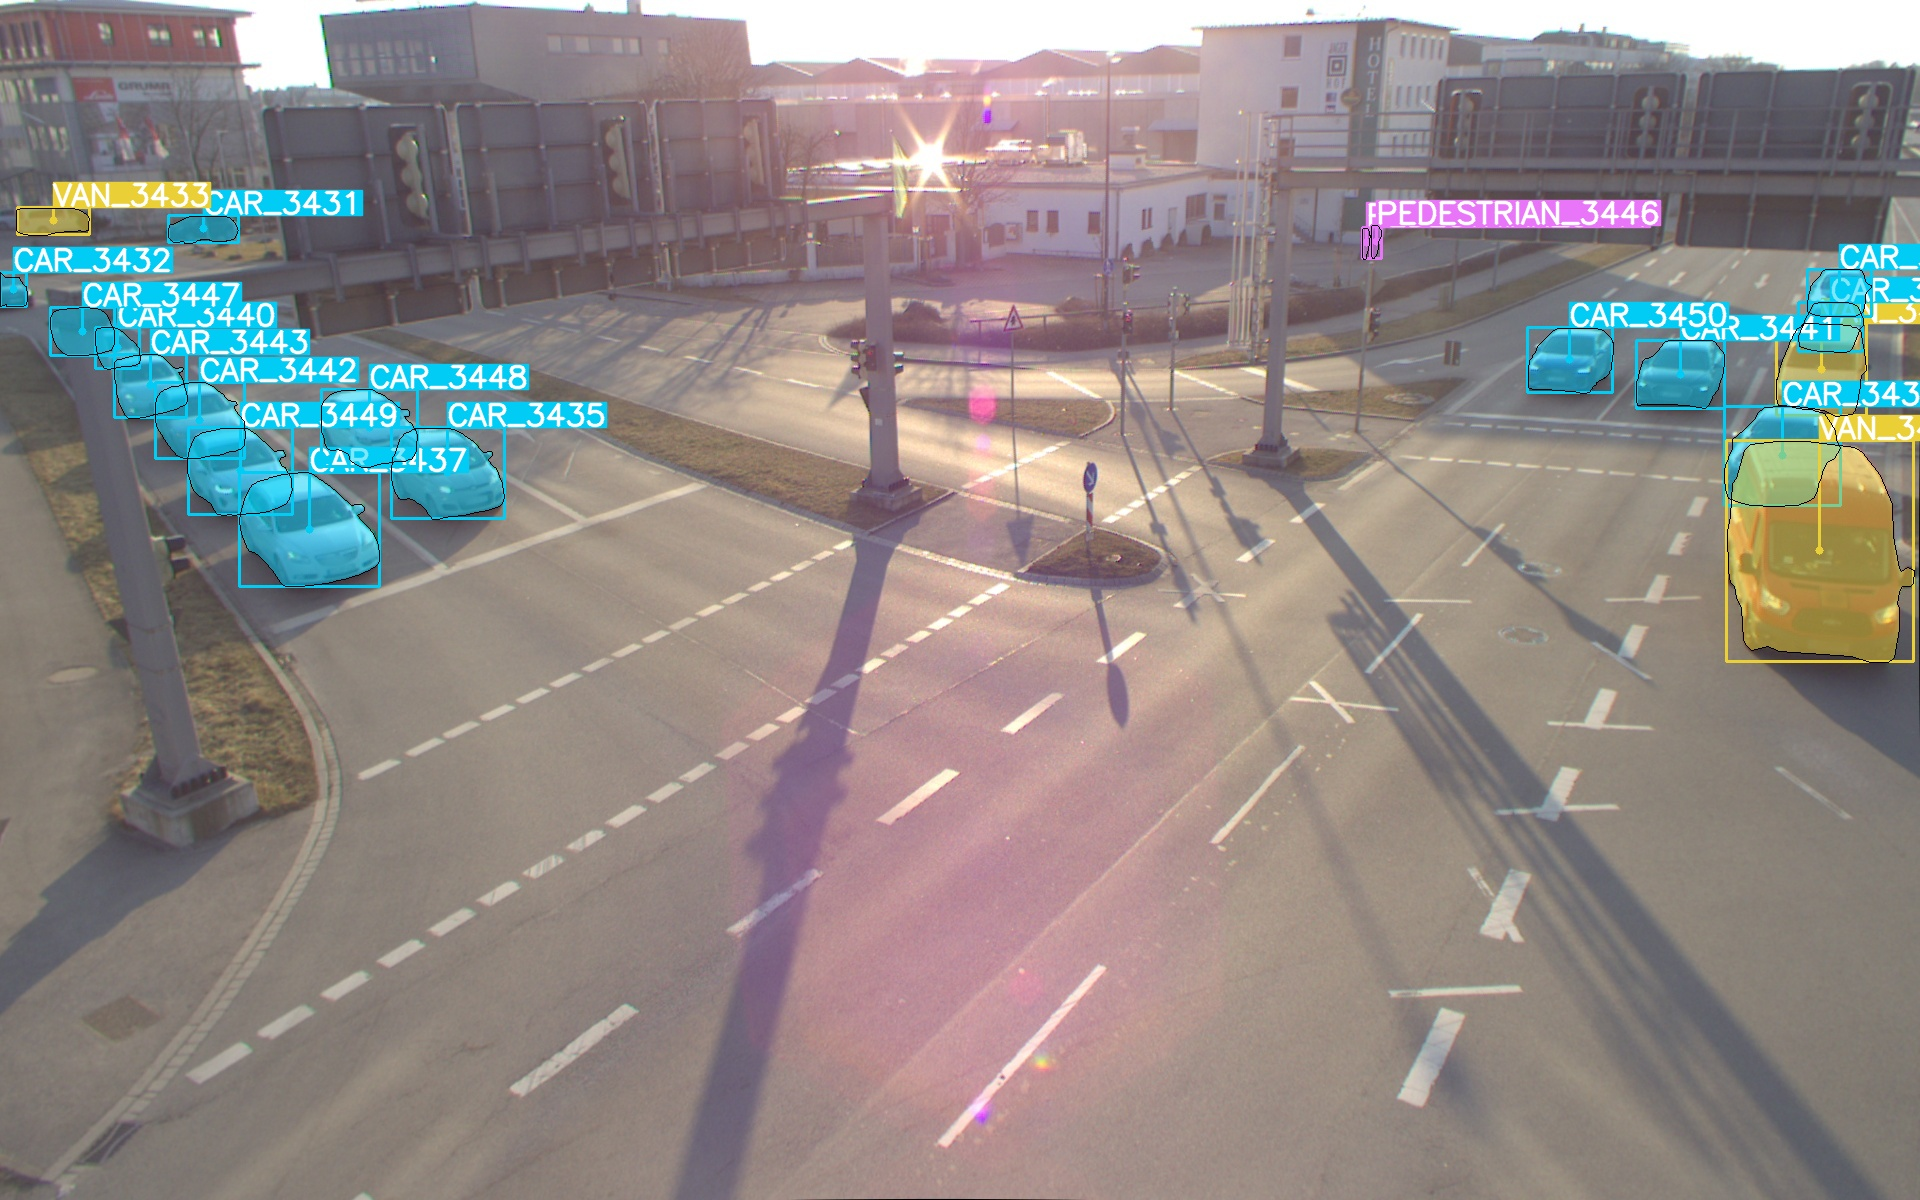
\includegraphics[width=\linewidth]{cvat_r02_s01_1.jpg}
		\vspace{-\baselineskip} % Remove space above image
	\end{subfigure}
	\begin{subfigure}{0.48\textwidth}
		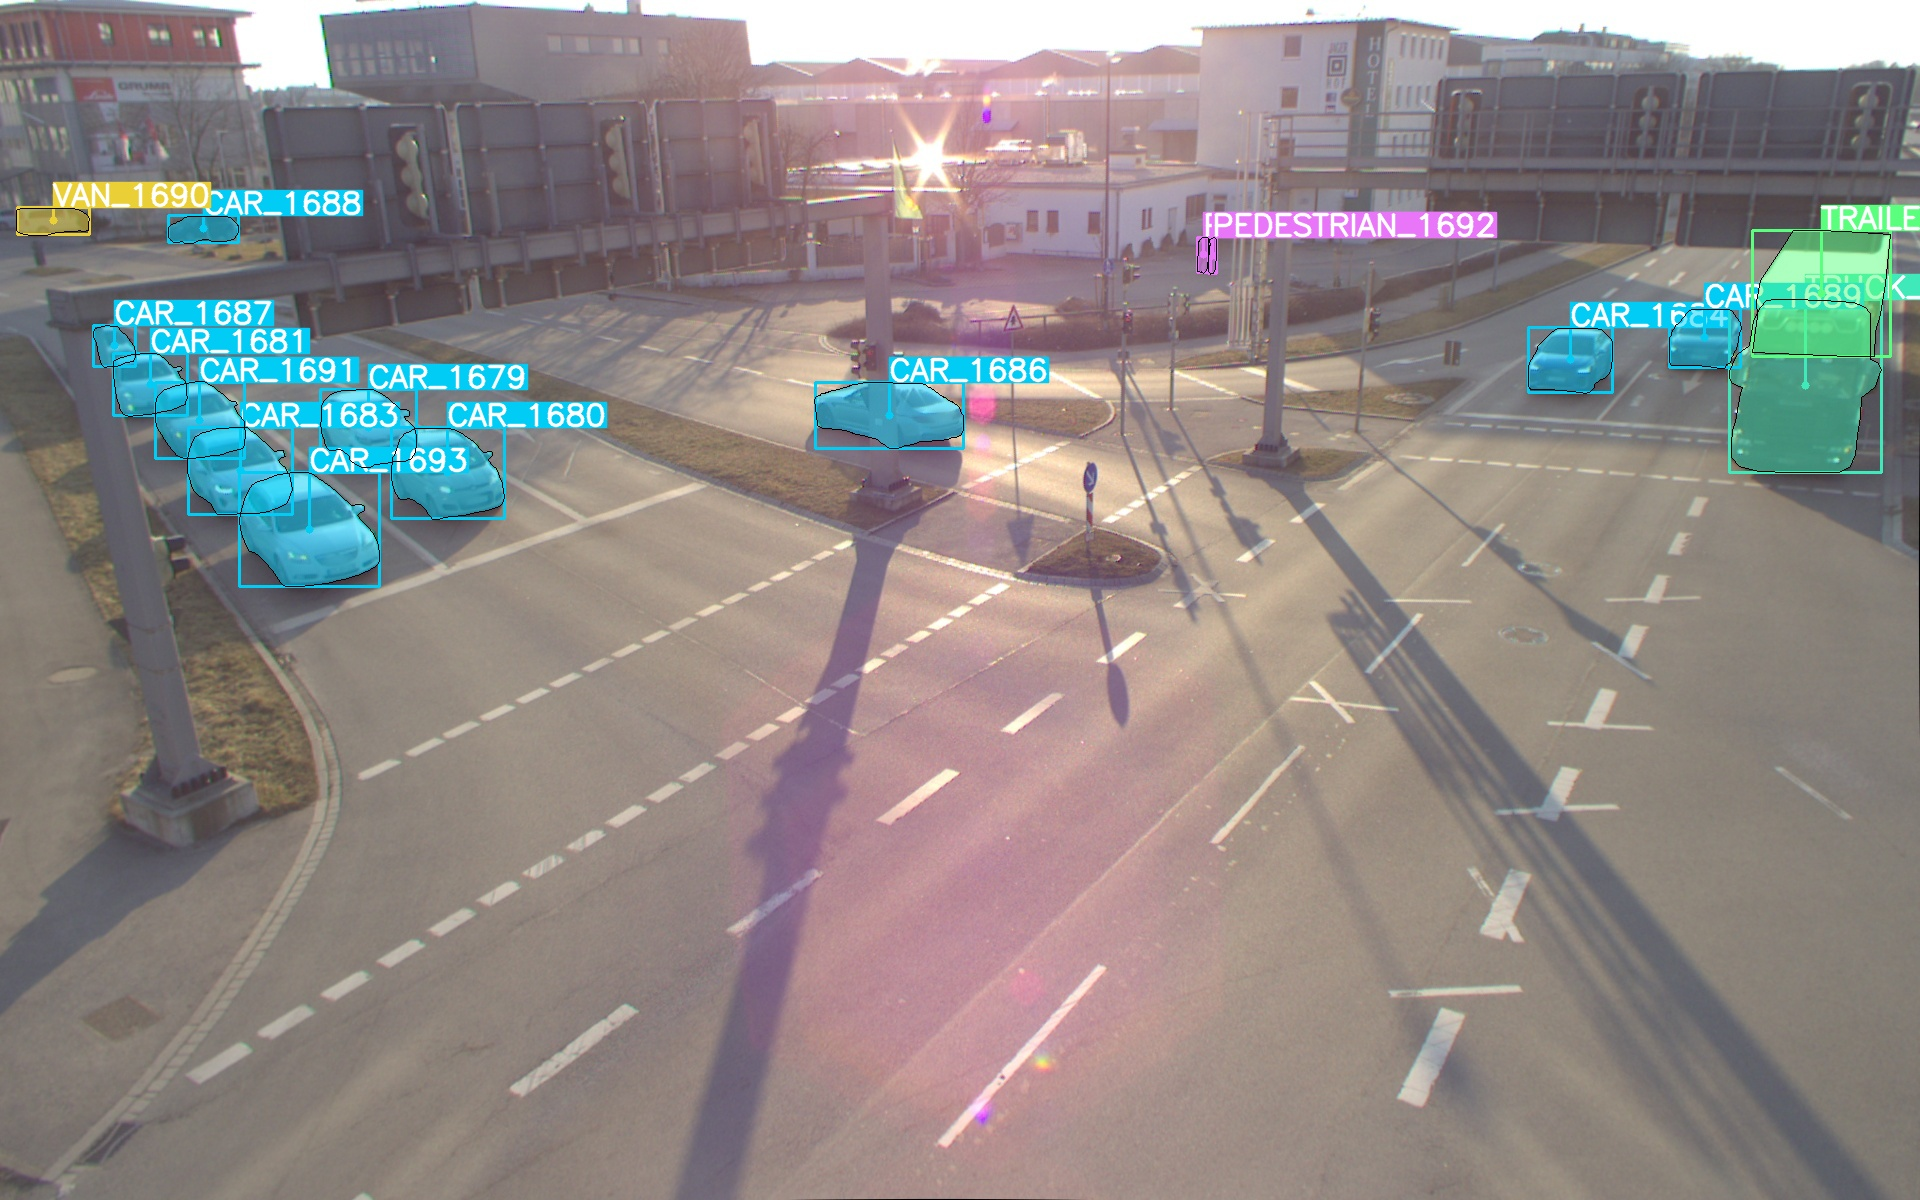
\includegraphics[width=\linewidth]{cvat_r02_s01_2.jpg}
		\vspace{-\baselineskip} % Remove space above image
	\end{subfigure}
	\vspace{-0.6em}
	\caption*{R02 S01 south1}
	
	%\vspace{-0.6em}
	
	% Second Column
	\begin{subfigure}{0.48\textwidth}
		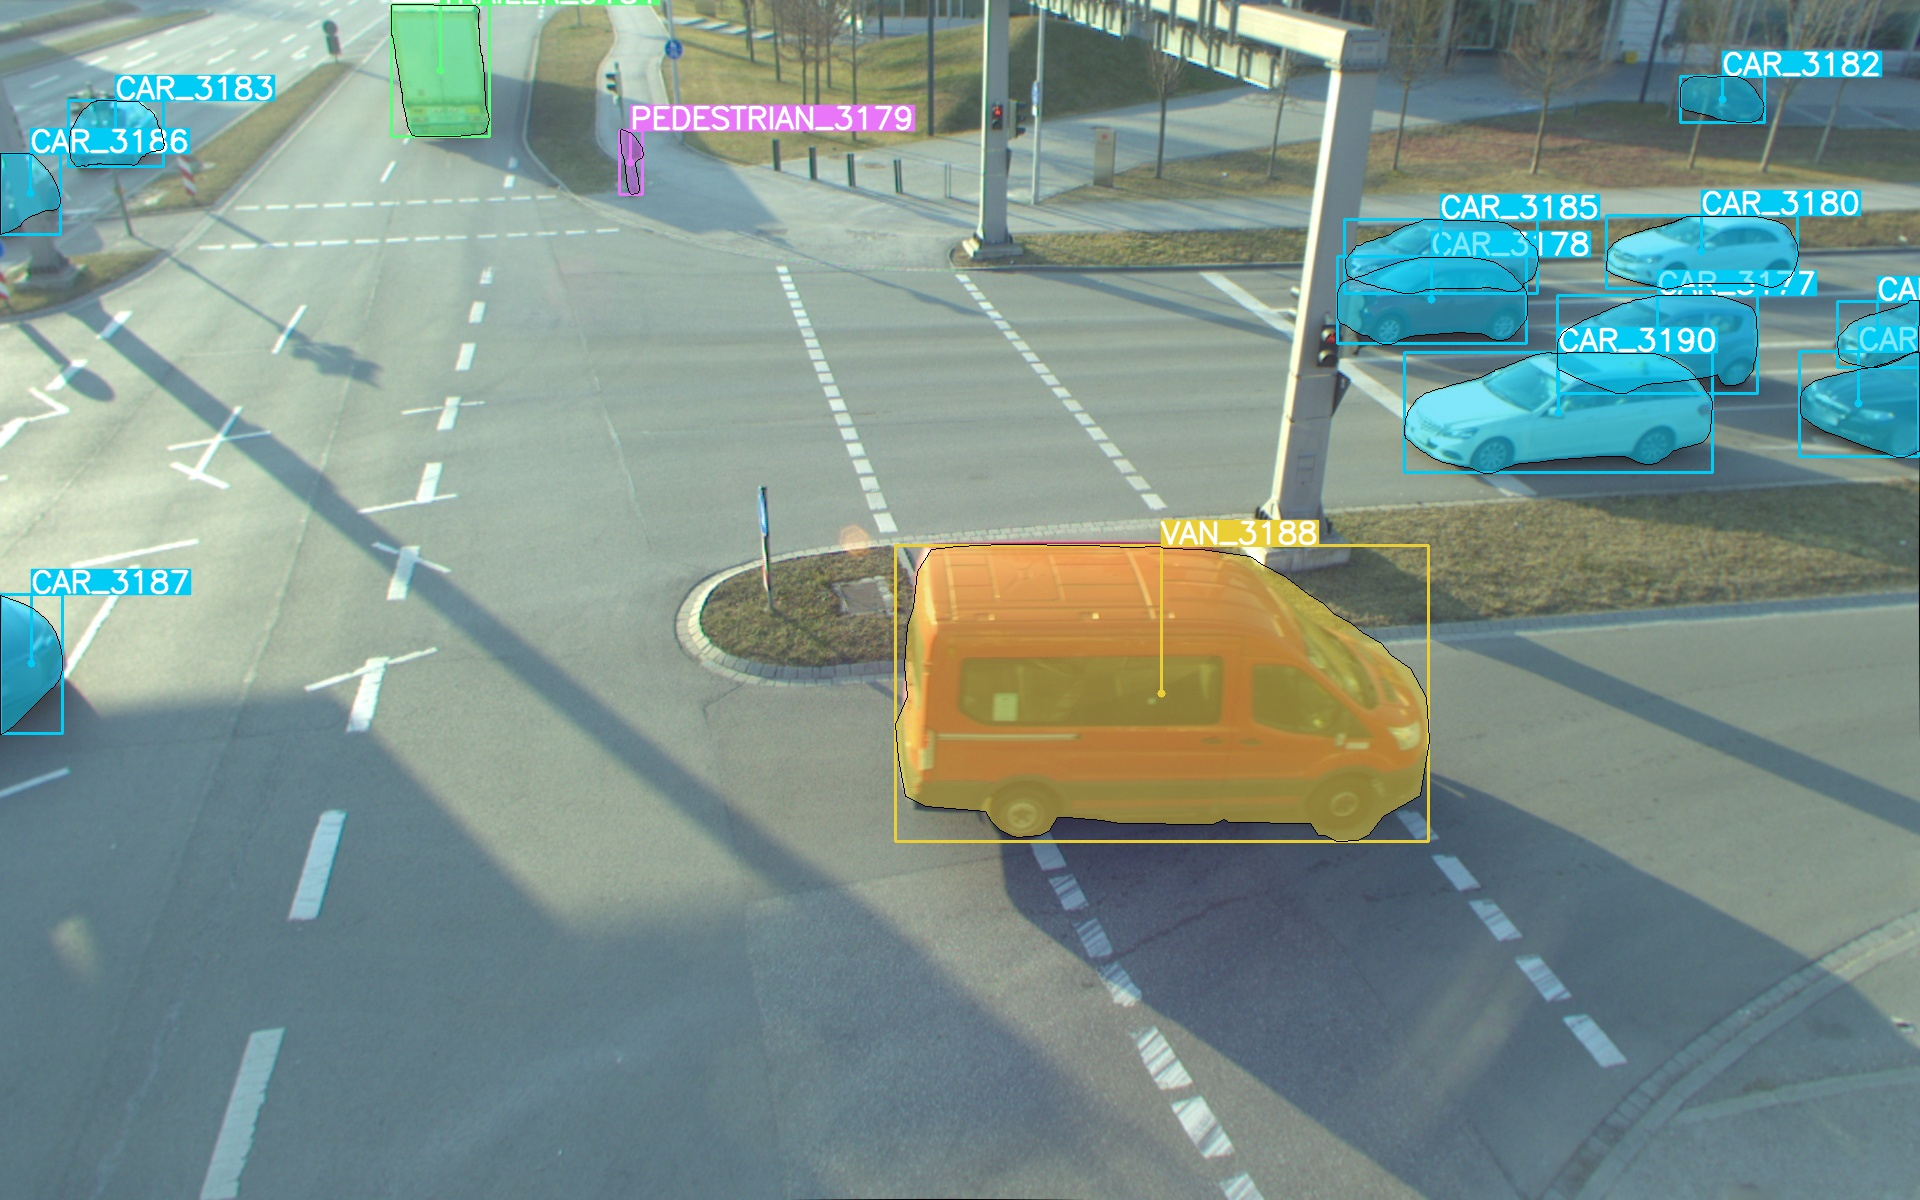
\includegraphics[width=\linewidth]{cvat_r02_s02_1.jpg}
		\vspace{-\baselineskip} % Remove space above image
	\end{subfigure}
	\begin{subfigure}{0.48\textwidth}
		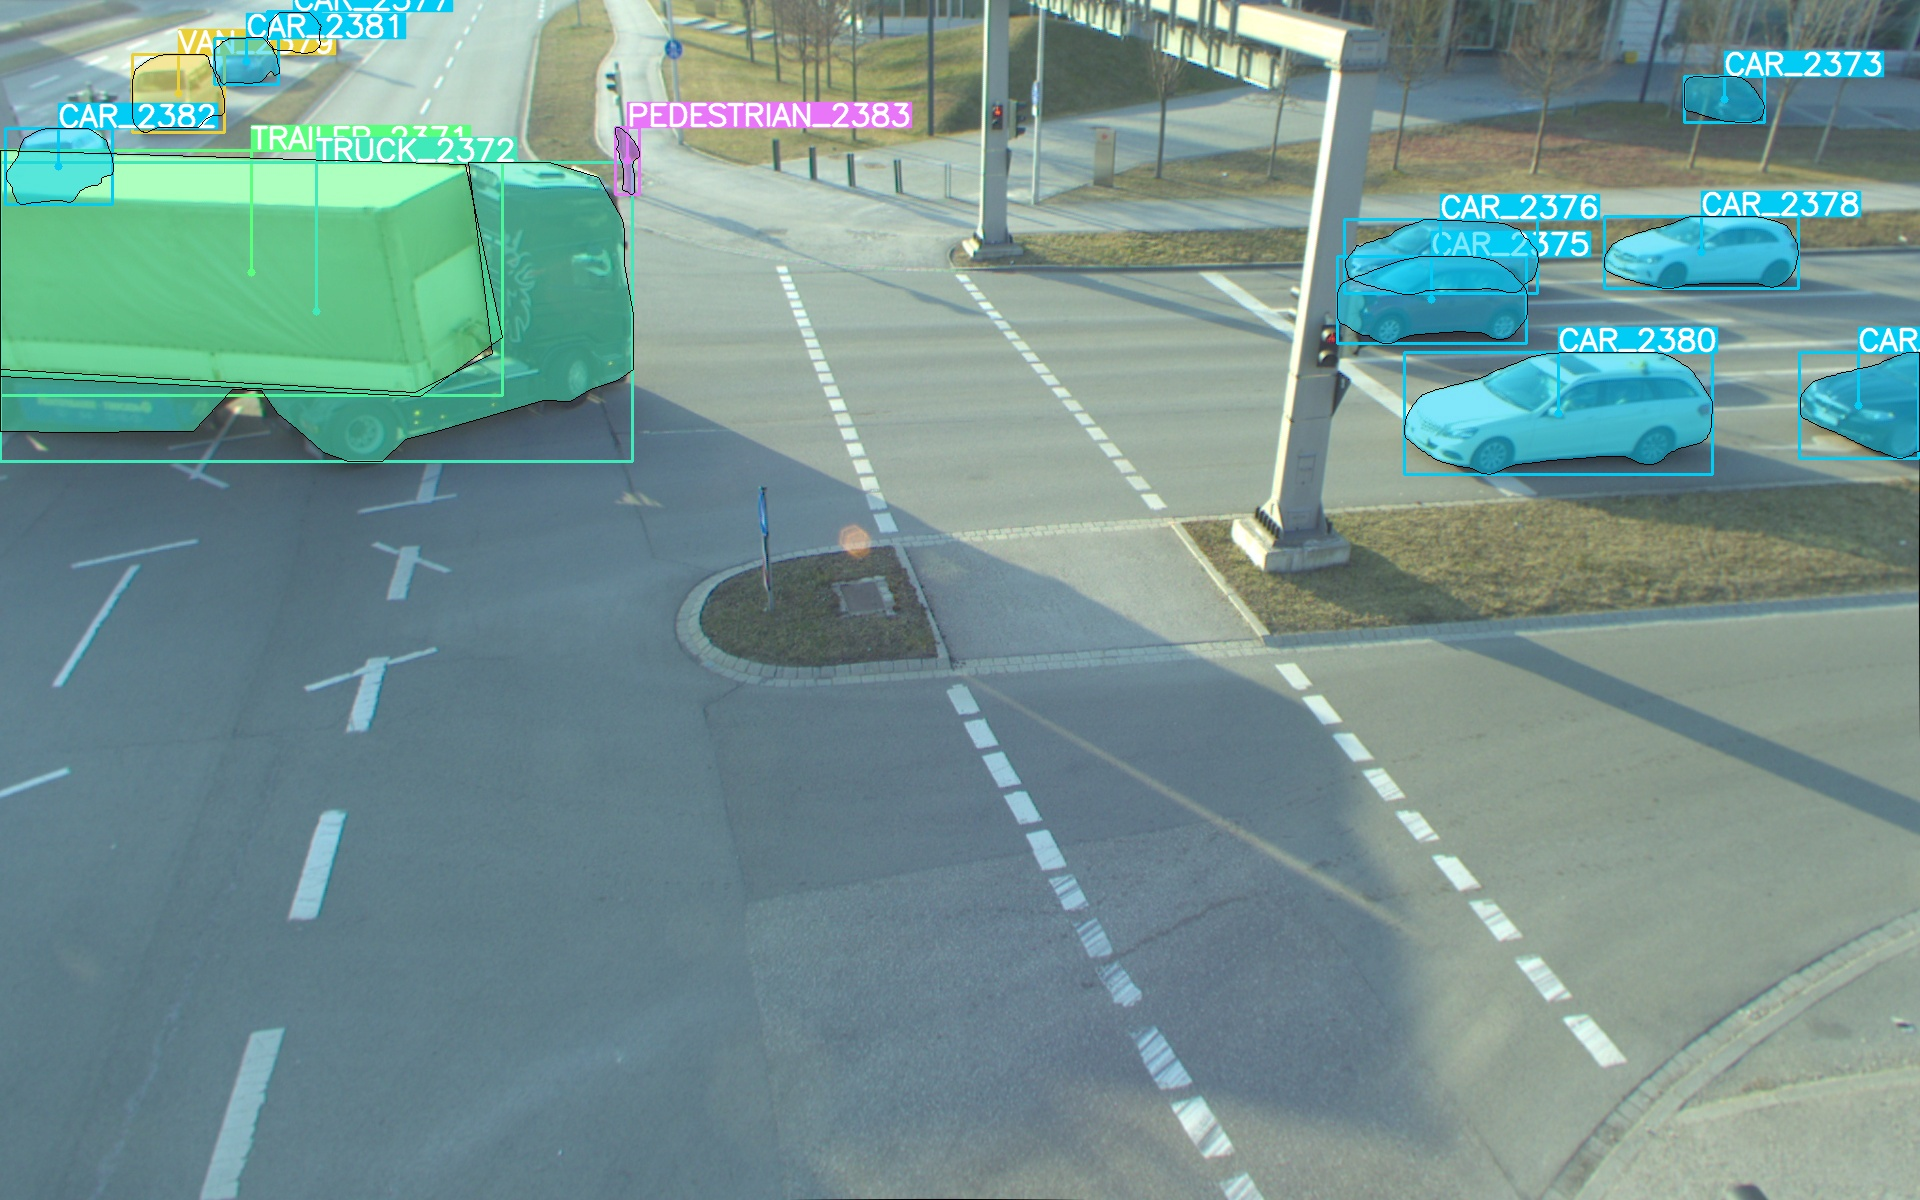
\includegraphics[width=\linewidth]{cvat_r02_s02_2.jpg}
		\vspace{-\baselineskip} % Remove space above image
	\end{subfigure}
	\vspace{-0.6em}
	\caption*{R02 S01 south2}
	
	\caption{Four frames from release 02 sequence 01 of TUMTraf Dataset with the south1 and south2 camera, respectively. The frames are visualized with the object's full instance masks, full bounding boxes, and categories. The missing classes from COCO, like TRAILER and VAN, are also annotated.}
	\label{figure:cvat_annotated_example}
\end{figure}



\section{Instance Segmentation Node} \label{sec:object_detection_with_yolov8}

Similar to the Instance Segmentation Node of the Providentia Mono3D system, we implement a 2D detector node utilizing the YOLOv8 instance segmentation model. The interaction between the camera driver node and the 3D detection node remains unchanged. This 2D detector node receives full-resolution 1920x1200 RGB frames from shared memory and publishes the 2D detection results to the 3D detector through ROS. The input frames, however, are not downscaled before inference. Research has demonstrated that maintaining full resolution during inference yields significantly better performance compared to downsampling (as discussed in section 5.3).

The new library style of YOLOv8 has significantly simplified interaction with the model. Models in various formats, such as Pytorch (.pt) or TensorRT (.engine/.trt), can be loaded in the same way. After inference, we apply non-maximum suppression (NMS) with a threshold of 0.65 to filter out heavily overlapped detections. Subsequently, detections with lower confidence are filtered based on class-wise confidence thresholds. To differentiate between detection results of model weights trained on different datasets, including COCO, TUMTraf, and NuImages, the 2D detector node implements additional logic to correctly interpret category indices, utilizing different index-to-category mappings for each dataset.

For each input frame, the detector node publishes an output array of detected instances containing 2D bounding boxes, 2D segmentation masks, and confidence scores to downstream processes. The detected 2D segmentation instance masks can currently be transmitted in two formats: bit-packed masks or polygon contours. The former utilizes bit-packing to serialize pixel mask arrays for each instance. This results in 1920*1200 pixels per frame for full resolution, with each pixel being one bit, resulting in a total of 285000 bytes per frame. Alternatively, the latter approach transmits only the image coordinates (x,y) of the polygon points of the detected mask's contour, with each x or y coordinate being an unsigned-8-bit integer, requiring only 2 bytes per point. Hence, up to 142500 polygon points can be sent before reaching the level of bit-packed masks. Considering that each frame typically contains 20 to 30 objects, allowing each object to use 4750 points to describe the polygon contour seems excessive. Therefore, we advocate for the second option as a better choice. However, since the current 3D detector expects bit-packed masks as input, a complete transition to polygon contours is not feasible yet. A future work would be to adjust the 3D detector's message reception to eliminate the need for sending bit-packed masks entirely.

Additionally, 2D visualizations and OpenLABEL detection files can generated for further analysis and debugging.

\subsection{Training different YOLOv8 models}

Training different YOLOv8 models is a crucial aspect of this work. We choose the YOLOv8x, the largest model that promises the best accuracy, and train different model weights and evaluate their performance on the TUMTraf Intersection Dataset as well as their general generalization capabilities. The above-mentioned annotated split of the TUMTraf Intersection Dataset is converted to YOLO's required data structure as preparation for training. 

We focus on training two main models. The first YOLOv8x model is trained from the annotated TUMTraf Intersection Dataset from scratch for a total of 300 epochs on a full image resolution of 1920. The second utilizes the pre-trained YOLOv8x model published by Ultralytics, which was initially trained on COCO with an image size of 640 for 500 epochs, and fine-tunes it on the TUMTraf Intersection Dataset with an image size of 1920. Both models demonstrate improved performance in both 2D and the subsequent 3D detections. Particularly noteworthy is the first model trained on TUMTraf from scratch, which not only outperforms the existing 2D detector based on YOLOv7 on the TUMTraf Intersection Dataset but also exhibits superior generalization to other scenarios, such as nighttime and highway scenes. Compared to YOLOv7, it achieves a 2D mAP@[.5:.95] difference of over 18\% and a 3D mAP@[.10] difference of almost 8\%. Further details of the evaluations are elaborated in \cref{chap:five}. 

Additionally, we fine-tune a model on the TUMTraf Intersection Dataset at a resolution of 640 to validate that training and detecting from higher image resolutions yield higher detection accuracy. In particular, the model weight with the highest accuracy at resolution 640 still performs approximately 16.5\% worse than the model weight with the highest accuracy at resolution 1920. 

To further enhance performance, we want to explore nuImages for pre-training. As described in \Cref{section:segmentation_dataset}, nuImages is a significantly larger dataset compared to COCO, making it a potentially better candidate for pre-training. However, due to its immense size, training on nuImages requires more time per epoch and may require many epochs to converge. Following the training of the YOLOv8x model from scratch on nuImages with a resolution of 1280 for 50 epochs, we assess its performance. It is evident that pre-training on nuImages for 50 epochs is not enough to yield any improvement compared to the published model pre-trained on COCO. We are currently continuing the training of this model in pursuit of improved results.

\subsection{TensorRT Optimization}

To preserve the real-time performance of the Providentia system, we export the models to TensorRT for accelerating inference. NVIDIA’s TensorRT  \cite{vanholder2016efficient} is a high-performance deep-learning inference library designed to optimize and accelerate the inference of deep neural networks on NVIDIA GPUs. It employs various techniques, such as weight and activation precision calibration, to achieve FP32, FP16, or INT8 quantization with a significantly lower model footprint. Layer and tensor fusion, combined with kernel auto-tuning, further maximizes the GPU utilization. We exported the model using FP16 quantization and optimized it for inference on TUMTraf full-resolution frames of size 1920.

The exportation of the YOLOv8x model from Pytorch to TensorRT format significantly boosts the inference speed, nearly tripling it from 10 frames-per-second (FPS) to 28 FPS for inference at an image resolution of 1920x1920, and from 66 FPS to 200 FPS for an image resolution of 640x640.

\subsection{Training C2F model}

Since the YOLOv8x model trained on the TUM Traffic Intersection dataset from scratch has achieved the best performance improvement in visible 2D segmentation, we leverage its detections to extend them to amodal masks using the C2F-seg model. First, we adapt and fine-tune the C2F-seg amodal segmentation model on the TUMTraf Intersection Dataset. Subsequently, we give it the visible detections as inputs and generate amodal detections, which are then passed to the subsequent 3D detector to produce the final 3D bounding boxes.

It is intriguing to explore whether the additional information provided by amodal masks can enhance the final 3D perception results. However, the results are somewhat surprising; despite receiving visible detections from the YOLO model as input, the C2F model achieves a lower improvement in 3D performance (only 1.90\% compared to the 7.53\% improvement of YOLOv8x trained on TUMTraf Intersection). This suggests that extending to amodal masks using C2F has even worsened the final 3D perception performance. Further in-depth analysis of this phenomenon would be valuable to uncover the underlying reasons.
% why? Amodal mask makes the 3D bbox bigger and increases FP by eval against ground truth? 

Additionally, regarding inference time, C2F requires, on average, around 22 milliseconds to extend one visible mask to an amodal mask. For a frame containing 20 objects, this would add an additional 440 milliseconds on top of the visible segmentation time. There may be potential for improvement when C2F can be exported to TensorRT in future work.
